\chapter{Deterministic Chaos vs. Stochastic Turbulence}
\label{c_chaos}

In this chapter, I tackle the difficult question regarding the level of determinism of the turbulence in LAPD. Through the previous chapters, I maintained the modern 
Ruelle and Takens~\cite{ruelle1971} viewpoint that the turbulence is governed by a set of deterministic differential equations. That allowed me to simulate the turbulence using a set of differential
equations with non-random coefficients. However, I also largely used statistical and structural theory to diagnose the turbulence, assuming as most do, that the large number of degrees of freedom
available to the turbulence prevents a simpler diagnosis.
In this chapter, I explore this assumption regarding the number of relevant degrees of freedom, which is equivalent to the question of whether the turbulence in LAPD is deterministic
(governed by a few degrees of freedom) or stochastic (governed by many).
I am motivated by the recent work on LAPD by Pace, Shi, Maggs, and Morales
~\cite{pace2008a,pace2008b,shi2009,maggs2011,maggs2012a,maggs2012b,maggs2013}, which I review below. Their conjecture is that the plasma turbulence in LAPD and a number of other devices is deterministic.

\section{Lorentzian Pulses as an Indicator of Deterministic Chaos}
\label{s_lorentzian_pulses}

\begin{figure}[!ht]
\centerline{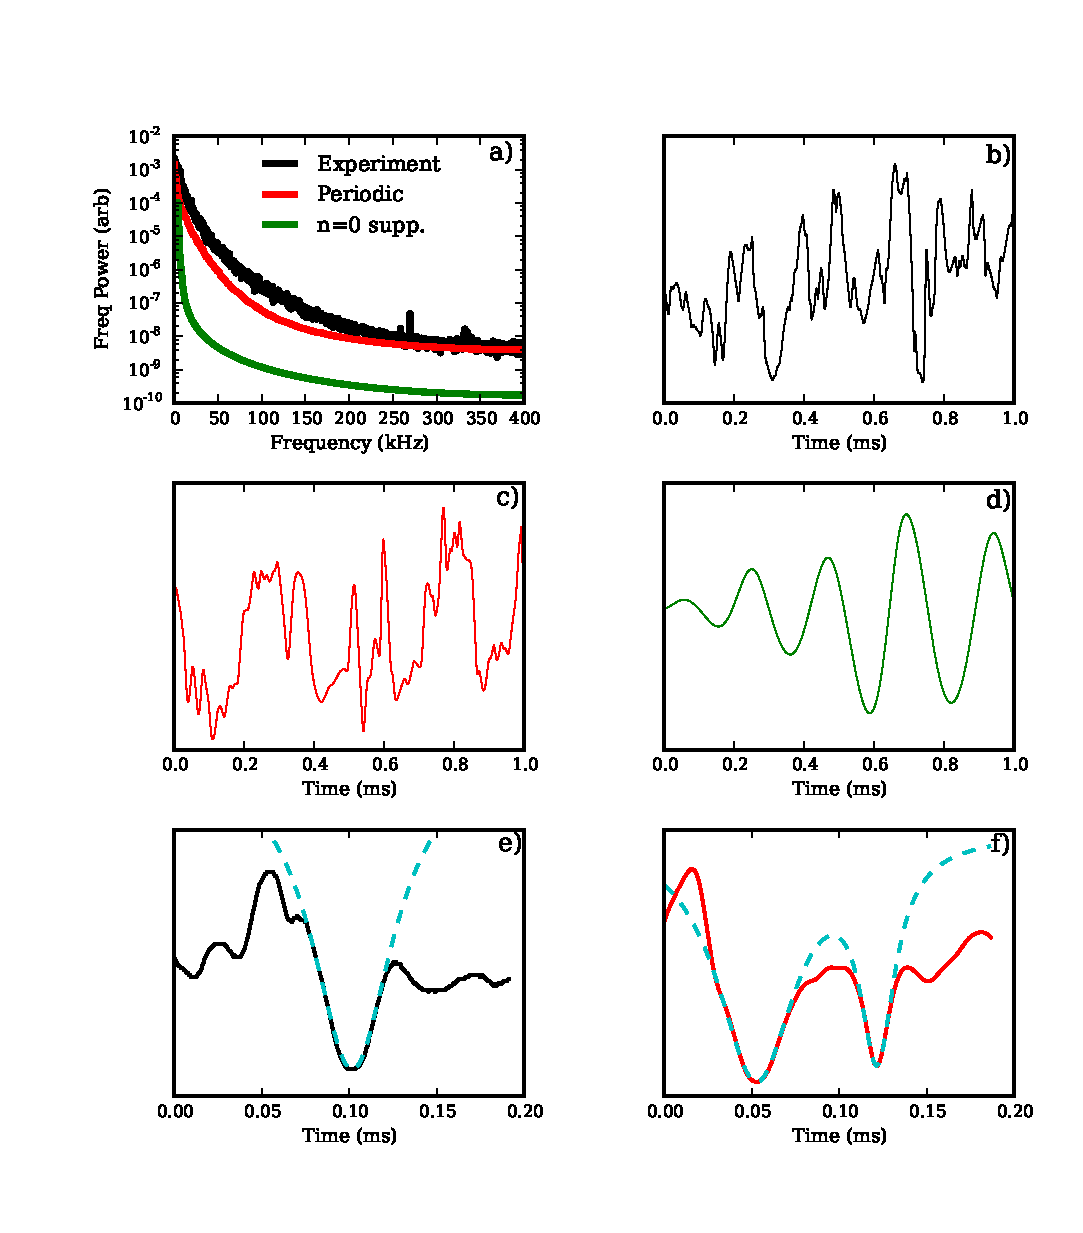
\includegraphics[]{lorentzians}}
\caption{Lorentzian pulses in time signals}
\label{lorentzians}
\end{figure}


In this section, I explain some of the work by Pace, Shi, Maggs, and Morales, in which they identified exponential frequency spectra and 
Lorentzian pulses in the time signals of experimental measurements, leading them to the turbulence as deterministic chaos.
I do this while applying their findings to my experimental and simulation data, which should not be too much different than some of the data they used, especially that of Pace~\cite{pace2008a,pace2008b}.

Since they based most of their analysis and findings on time signals of experimental data rather than spatially resolved simulation data, 
I restrict myself here to looking at density and $I_{sat}$ time signals, neglecting simulated spatial structures.
While comparing time signals point for point is futile in chaotic systems due to sensitivity to initial conditions,
chaotic systems can produce time signals with identifiable visual characteristics.
In this regard, Pace et al. discovered that the time signals in LAPD experiments and in the edge of some magnetic confinement devices
are made up of Lorentzian-shaped pulses~\cite{pace2008a,pace2008b}. A Lorentzian is simply a function of the form

\beq
\label{lorentz_eqn}
f(t) = A/\left[1 + (t - t_0)^2/\tau^2 \right]
\eeq
where $A$ is the pulse amplitude, $t_0$ is its center, and $\tau$ is the pulse width. The absolute value of the Fourier transform of a Lorentzian is simply a decaying exponential, so
the Lorentzian pulses in the time signals lead to frequency power spectra that have exponential shape, which show up as a straight line in a log-linear plot. In such a plot, the slope of the line
is proportional to the Lorentzian width $\tau$. Sometimes, however, the Lorentzian
pulses in the time signals have different widths, which cause different spectral slopes, leading to power spectra with non-exponential shape. 

To compare my time signals to those of Pace and others, I first plot the frequency spectra of the experiment,
the Periodic simulation, and the $n=0$ suppressed simulation in Fig.~\ref{lorentzians} a). I don't use any window functions since they can distort any structures in the time signals,
and I use only one radial location (30 cm) rather than doing a volume average. Clearly, the spectra are not exponential for either the experiment or the simulations. This doesn't rule out
Lorentzian pulses in the time signals, however, as long as the time signals have pulses of varying width. So next, I look at the time signals of the experiment and simulations. I show representative
signals for the experiment, Periodic simulation, and $n=0$ suppressed simulation in Figs.~\ref{lorentzians} b), c), and d), respectively. Notice that the experiment and Periodic simulation
appear to have qualitatively similar time signals, while the $n=0$ suppressed simulation has a much different, simpler looking signal. Furthermore, the experiment and Periodic simulation contain
a number of pulse-like features. I take a closer look at some of these pulses in Figs.~\ref{lorentzians} e) (experiment) and f) (Periodic simulation), trying to find times when the pulses
are relatively isolated. In Fig.~\ref{lorentzians} e), I fit one of these pulses to a Lorentzian function (the dashed line), 
proving that this pulse, does in fact have a Lorentzian shape. I confirm that a Lorentzian does provide a better fit than a Gaussian, which doesn't fit the pulse as well for as long of a time
range as the Lorentzian. Furthermore, Gaussian pulses create spectra that look very different from those in Fig.~\ref{lorentzians} a), supporting the claim that the pulses have Lorentzian
rather than Gaussian shape. Finally, in Fig.~\ref{lorentzians} f),
I look at a signal snipet from the Periodic simulation with two relatively isolated pulses, and I fit a sum of two Lorentzian functions to this. Clearly, the fit is excellent as
both of these pulses have Lorentzian shape, and importantly, they have different widths, explaining the non-exponential shape of the spectra. I don't show a fit to the $n=0$ suppressed simulation
signal, but I note that it is quite sinusoidal with seemingly two or so dominant low frequency waves, which is clear from the highly peaked, non-broadband frequency spectra.

Now the reason why Lorentzian pulses show up in the time signals was explained by Maggs and Morales~\cite{maggs2012a}. They showed that some chaotic nonlinear systems -- including the well-known
Lorenz system~\cite{lorenz1963} -- undergo a certain kind of bifurcation, which they called a Lorentzian bifurcation. That is, some systems undergo a bifurcation from a solution that settles
on a limit cycle attractor to a solution that settles on a chaotic strange attractor, in which one of the variables has a trajectory made of Lorentzian pulses.
In a plasma, that trajectory is associated with an ${\bf E \times B}$ flow, which advects the scalar density and temperature, imprinting the Lorentzian shape onto their time signals.
The fact that experimental signals are made up of Lorentzian pulses, they say, indicates that the systems are deterministic and not stochastic because the systems are close to the bifurcation point
between the limit cycle and the strange attractor.

To understand this last important point, note that in general, dynamical systems have some control parameter associated with them that determines their steady state behavior. For instance, 
nuetral fluid behavior is often determined by the Reynolds number. As the control parameter increases, the system undergoes a series of bifurcations in which each bifurcation increases the effective
phase space dimension of the attractor. A limit cycle is a two-dimensional attractor. Strange attractors often have fractional dimension greater than two~\cite{manneville2004}.
The bifurcation from a limit cycle attractor to strange attractor then increases the dimension, or equivalently increases the effective number of degrees of freedom available to the system.
As the bifurcation parameter increases still further, the number of effective degrees of freedom increases, eventually becoming high enough for the system to be more stochastic than deterministic.
Any system then, near the bifurcation point between limit cycle and strange attractors will have a small number of degrees of freedom, making it deterministic.

For LAPD and similar plasma systems, the control parameters ought to be proportional to the equilibrium gradients. 
For the system to display Lorentzian chaotic dynamics, the conjecture is that the control parameter and thus the gradient must be high enough so that the attractor is not
a limit cycle, but low enough so that it still has a Lorentzian trajectory associated with it.
Furthermore, such a situation may be a natural consequence of chaotic advection in confinement-like systems because chaos causes
transport which relaxes the gradients and prevents them from building up. The control parameter, thereforem should not be able to grow much beyond the point where chaos ensues. 
In other words, the control parameter
causes the chaos, but the chaos regulates the the control parameter, preventing the system from straying from the bifurcation point between the limit cycle and the low dimensional strange attractor.

\section{Permutation entropy as an Indicator of Chaos}
\label{s_ent_comp}

While Lorentzian pulses in the time signals of experimental data provided the clue to the possible chaotic nature of the turbulence in LAPD, there are more direct and more conclusive ways
to determine how deterministic versus how stochastic a system is. Therefore, Maggs and Morales set out to test one of their LAPD experiments with one of these more direct methods~\cite{maggs2013},
namely a method invented by Bandt and Pompe about a decade ago~\cite{bandt2002}. The Bandt-Pompe method, called permutation entropy, uses a
time signal of a single observable to quantify the amount of determinism of the underlying process that creates the time signal. The method has gained better theoretical
interpretation over the years, and various researchers have refined its implementation. Recently, Riedl et al.~\cite{riedle2013} published a review on permutation entropy that provides theory,
instructions, and most importantly, practical considerations for using the Bandt-Pompe method. In light of this review based on dozens of researchers' experience, I follow the procedures and lessons
in it rather than those in the Maggs and Morales paper.

\subsection{Trajectory reconstruction by the method of delays}
\label{ss_delays}

The Bandt-Pompe permutation entropy is partly based on a standard chaotic time signal analysis technique that is often called the method of delays, 
first formalized by Takens~\cite{takens1981}. The method of delays attempts to reconstruct the trajectory of an attractor on a manifold in the phase space over which the effective dynamics
take place. I review the method following Manneville's treatment~\cite{manneville2004}, but I note that there is another nice review that is more freely available by Theiler~\cite{theiler1990}.

First, one can formally write the dynamical system $\mathbf{\dot{X}} = \mathbf{\mathcal{F}} (\mathbf{X})$ for the state $\mathbf{X}$ in the phase space $\mathbb{X}$. Furthermore,
there is a manifold $\mathbb{M}$ of dimension $d_{\rm{eff}}$ on which the dynamics lie, where  $d_{\rm{eff}}$ is less than the dimension of the entire space $\mathbb{X}$. The only available
information is the time signal $W$ that is measured in an experiment. 
It is some unknown projection of the state $\mathbf{X}$ onto a single dimension: $W = \mathcal{W} ({\mathbf{X}})$. 
For a discrete time signal, the dynamical system may be approximated as

\beq
\label{dyn_sys_approx}
{\mathbf{X}}_{k+1} = {\mathbf{\mathcal{F}}} ({\mathbf{X}}_k)
\eeq
where the subscript denotes a time index. Reconstructing the dynamics amounts to determining an empirical relation between the ${\mathbf{X}}_k$ in their phase space and the observables
$W_k, k=0,1, \ldots$ Clearly, $W_0 = {\mathcal{W}}({\mathbf{X}}_0)$ is not sufficient to determine ${\mathbf{X}}_0$ since one coordinate is not enough to define ${\mathbf{X}}_0$. But, note that
$W_1$ is to the projection of ${\mathbf{X}}_1$, which evolves from ${\mathbf{X}}_0$ under the map $\mathbf{\mathcal{F}}$. Thus, the second measurement $W_1$ adds a piece of information
about the coordinate ${\mathbf{X}}_0$ through $W_1 = {\mathcal{W}}({\mathbf{X}}_1) = {\mathcal{W}}({\mathcal{\mathbf{F}}} ({\mathbf{X}}_0))$. The third measurement, $W_2$ further provides information
on ${\mathbf{X}}_0$ through $W_2 = {\mathcal{W}}(\mathcal{\mathbf{F}} (\mathcal{\mathbf{F}} ({\mathbf{X}}_0)))$. 
In principle, a sufficiently long array of measurements of length $d_{\rm{test}}$, $\{W_0, W_1, \ldots , W_{d_{\rm{test}}-1}\}$ should serve to specify
${\mathbf{X}}_0$. Similarly, $\{W_1, \ldots , W_{d_{\rm{test}}}\}$ specifies ${\mathbf{X}}_1$, etc. 
Eventually, a whole trajectory ${\mathbf{X}}_k, k=0,1,\ldots$ can be reconstructed from the series of vectors,
${\mathbf{V}}_k = \{W_k, \ldots , W_{k+d_{\rm{test}}-1}\}$, existing in ${\mathbb{R}}^{d_{\rm{test}}}$.

The length $d_{\rm{test}}$ of the reconstruction vectors can be increased until the method produces a reliable reconstruction of the trajectory. $d_{\rm{test}}$ must be large enough so that one does
not lose any useful dynamical information. This means that different states must also have different reconstructions:

\beq
\label{diff_recons}
{\mathbf{X}}_k \ne {\mathbf{X}}_{k'} \rightarrow {\mathbf{V}}_k \ne {\mathbf{V}}_{k'}
\eeq

The tentative number $d_{\rm{test}}$ of components used to reconstruct the state vectors is more properly regarded as the effective dimension of the space in which the effective phase space
can be imbedded by means of an injective map. Thus, I change notation from $d_{\rm{test}}$ to $d_e$, the embedding dimension. Takens theorem states that the ${\mathbf{V}}_k$ achieve
a reliable reconstruction provided that the $d_e$ are large enough: $d_e \ge 2 d_{\rm{eff}} + 1$. In chaotic systems, strange attractors often have fractal dimension, $d_f$, and one can
replace $d_{\rm{eff}}$ by $d_f$ in this inequality.

Moreover, the ${\mathbf{V}}_k$ can actually be any series of $d_e$ measurements, namely, ${\mathbf{V}}_k = [W_k, W_{k + \kappa_1}, \ldots, W_{k + \kappa_{d_e-1}}]$, where the $\kappa_q$ can take on
any values. It's natural to take the $\kappa_q$ as multiples of some basic $\kappa$ so that ${\mathbf{V}}_k = [W_k, W_{k + \tau}, \ldots, W_{k + (d_e-1)\tau}]$, where $\tau$ is the subsampling
rate.

In practice, the usefulness of the method of delays relies upon choosing optimal values for the two basic ingredients in the reconstruction: 
the embedding dimension $d_e$ and the subsampling rate $\tau$ ($\tau$ is really a time, not a rate). 
Optimal values can reduce the effects of noise on results and can minimize required computation and required length of time signals.
The generally accepted optimal choice for the subsampling rate $\tau$ is the time over which a signal becomes decorrelated with itself~\cite{manneville2004,riedle2013}.
While the autocorrelation time seems like a natural quantity to use, it doesn't always lead to a satisfactory choice of $\tau$. A better criterion resting on solid theoretical arguments
revoles around the use of a quantity called the mutual information, which is defined as

\beq
\label{mutual_info}
I_{mut}(\tau) = \sum_{W',W''} P_{\tau}(W',W'') \rm{ln} \left( \frac{P_{\tau}(W',W'')}{P(W') P(W''))}  \right)
\eeq
where $W' = W_k, W'' = W_{k+\tau}$, $P(W)$ is the probability distribution of the time signal $W$, and $P(W',W'')$ is the joint probability distribution function of the signals $W'$ and $W''$.
$I_{mut}(\tau)$ is a measure of the redundance in the signal. When $\tau$ is small, the signals $W'$ and $W''$ are highly correlated and $I_{mut}$ is large, but when $\tau$ is large and the
signals are uncorrelated, $P_{\tau}(W',W'')$ is essentially $P(W') P(W'')$, making $I_{mut}$ small.

\begin{figure}[!ht]
\centerline{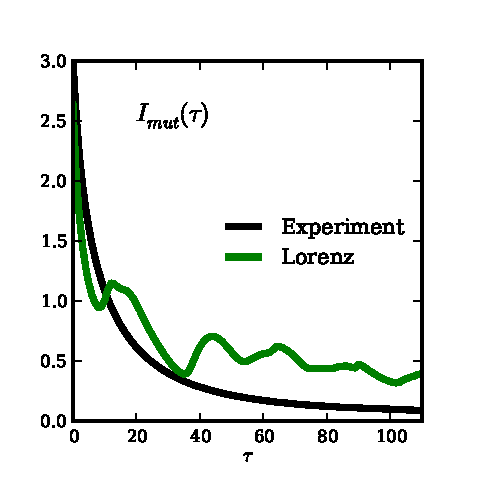
\includegraphics[]{imut}}
\caption{Mutual information as a function of subsampling rate}
\label{imut}
\end{figure}

In Fig.~\ref{imut}, I show an example of $I_{mut}(\tau)$ for two time signals. The black curve is the mutual information of the experimental $I_{sat}$ time signal at one radial location.
The green curve is the mutual information of the $x$ coordinate of the Lorenz model~\cite{lorenz1963}:

\beq
\label{lorenz_model}
\dot{x} = \sigma(y-x)   \qquad \dot{y} =  x(\rho-z) - y  \qquad \dot{z} = xy - \beta z
\eeq
where I use the well-know chaos-producing values $\sigma=10, \rho=28,$ and $\beta = 8/3$. I numerically solve the Lorenz model with an integration time step $0.017$ using a Python ODE solver.
The Lorenz model has an oscillating and decaying $I_{mut}(\tau)$, while the experiment has a simple decaying mutual information. The optimal value of $\tau$ corresponds to the first local minimum
of $I_{mut}$, which for the Lorenz model is at $\tau \approx 10$. The experiment has no local minimum, which can mean that there is either very large noise, the observable has been undersampled,
or that too many degrees of freedom are involved~\cite{manneville2004}. All of these can be a problem for using methods of low dimensional deterministic dynamical systems. However, in the next
section I review the permutation entropy, which can provide an optimal $\tau$ for the experiment. Furthermore, the permutation entropy can provide an optimal value for the embedding dimension
$d_e$. There are other methods for finding the optimal $d_e$, such as the method of false neighbors~\cite{manneville2004}, but I don't use it because it is difficult to analyze.

\subsection{Permutation Entropy}
\label{ss_pe}

The permutation entropy invented by Bandt and Pompe~\cite{bandt2002} defines a measure of the entropy of the time delay phase reconstructions based on their ordinal ranks. Specifically,
the time delay embedding vectors ${\mathbf{V}}_k$ with embedding dimension $n$ are binned into $n\!$ bins based on the order of their elements. For instance, if $n=3$ and the vector
${\mathbf{V}}_0 = (10,15,8)$, one counts this vector as one that has an ordinal representation of $(2,3,1)$. There are $3\!=6$ different possible permutations of the ranked vectors. 
The number of vectors of a given ordinal representation divided by the total number of embedding vectors produces a series of probabilities $p_j$ that add up to 1. The permutation entropy
is then defined by

\beq
\label{perm_ent}
P_n = - \sum_{j=1}^{n\!} p_j \rm{log}_2 (p_j)
\eeq
It is also convenient to define different normalizations for the permutation entropy, such as $h_n = P_n/(n-1)$, which allows for entropies with different $n$ to be compared, and
$H_n = P_n/\rm{log}_2 N$, which ranges from $0 \le H_n \le 1$.
